%%%%%%%%%%%%%%%%%%%%%%%%%%%%%%%%%%%%%%%%%%%%%%%%%%%%%%%%%%%%%%%%%%%%%%%%%%%%%%%
\section{Robustness with respect to time integration}
\label{sec:time-integrators}
%%%%%%%%%%%%%%%%%%%%%%%%%%%%%%%%%%%%%%%%%%%%%%%%%%%%%%%%%%%%%%%%%%%%%%%%%%%%%%%

The preceding mechanism was first identified with the implicit midpoint rule.
We now determine which parts belong to the spatial semidiscretization and which
are introduced by time stepping.  We compare implicit midpoint (the one-stage
Gauss method of order two), the two-stage Gauss--Legendre method of order four
(GL4), and the three-stage Gauss--Legendre method of order six (GL6).  In every
case the cubic-B-spline Petrov--Galerkin spatial operators are unchanged.  We
write
\begin{equation}
 \kappa=\frac{h}{c\Delta t},
\end{equation}
so that, for $c=1$, $\kappa$ is the number of time steps per compacton cell
crossing.  The forward-edge phase is fixed at $\phi_R=1/4$ in the spectral
comparisons.

\subsection{Time-refined Floquet spectrum}

For each integrator and each $(h,\kappa)$, we recompute the fully discrete
relative periodic compacton and its exact tangent one-cell map.  Independent
high-order reference values are obtained from the median of GL4 at
$\kappa=40,80$ and GL6 at $\kappa=10,20$:
\begin{equation}
 \rho_{F,\rm ref}=1.0958938054\quad(h=0.01),
 \qquad
 \rho_{F,\rm ref}=1.1342141857\quad(h=0.02),
 \label{eq:rho-time-ref}
\end{equation}
with reference-ensemble half ranges $8.9\times10^{-7}$ and
$3.0\times10^{-7}$, respectively.  Both limits lie well outside the unit
circle.  Hence the edge--Nyquist instability is a property of the spatial
semidiscretization and is not created by implicit midpoint.

At coarse temporal resolution, however, the integrator can modify both the
growth rate and the dominant branch.  For $h=0.01$ and $\kappa=5$, midpoint
gives a real flip multiplier $\lambda=-1.056633$, whereas GL4 and GL6 give
complex pairs with spectral radii $1.095665$ and $1.095920$, respectively.
For $h=0.02$ and $\kappa=20$, the corresponding radii are $1.130947$,
$1.134215$, and $1.134214$.  The relative periodic compacton profiles remain
nearly indistinguishable: the midpoint--GL4 $L^\infty$ differences are
$1.3\times10^{-8}$ and $9.6\times10^{-8}$ in the two principal cases.

\begin{figure}[t]
 \centering
 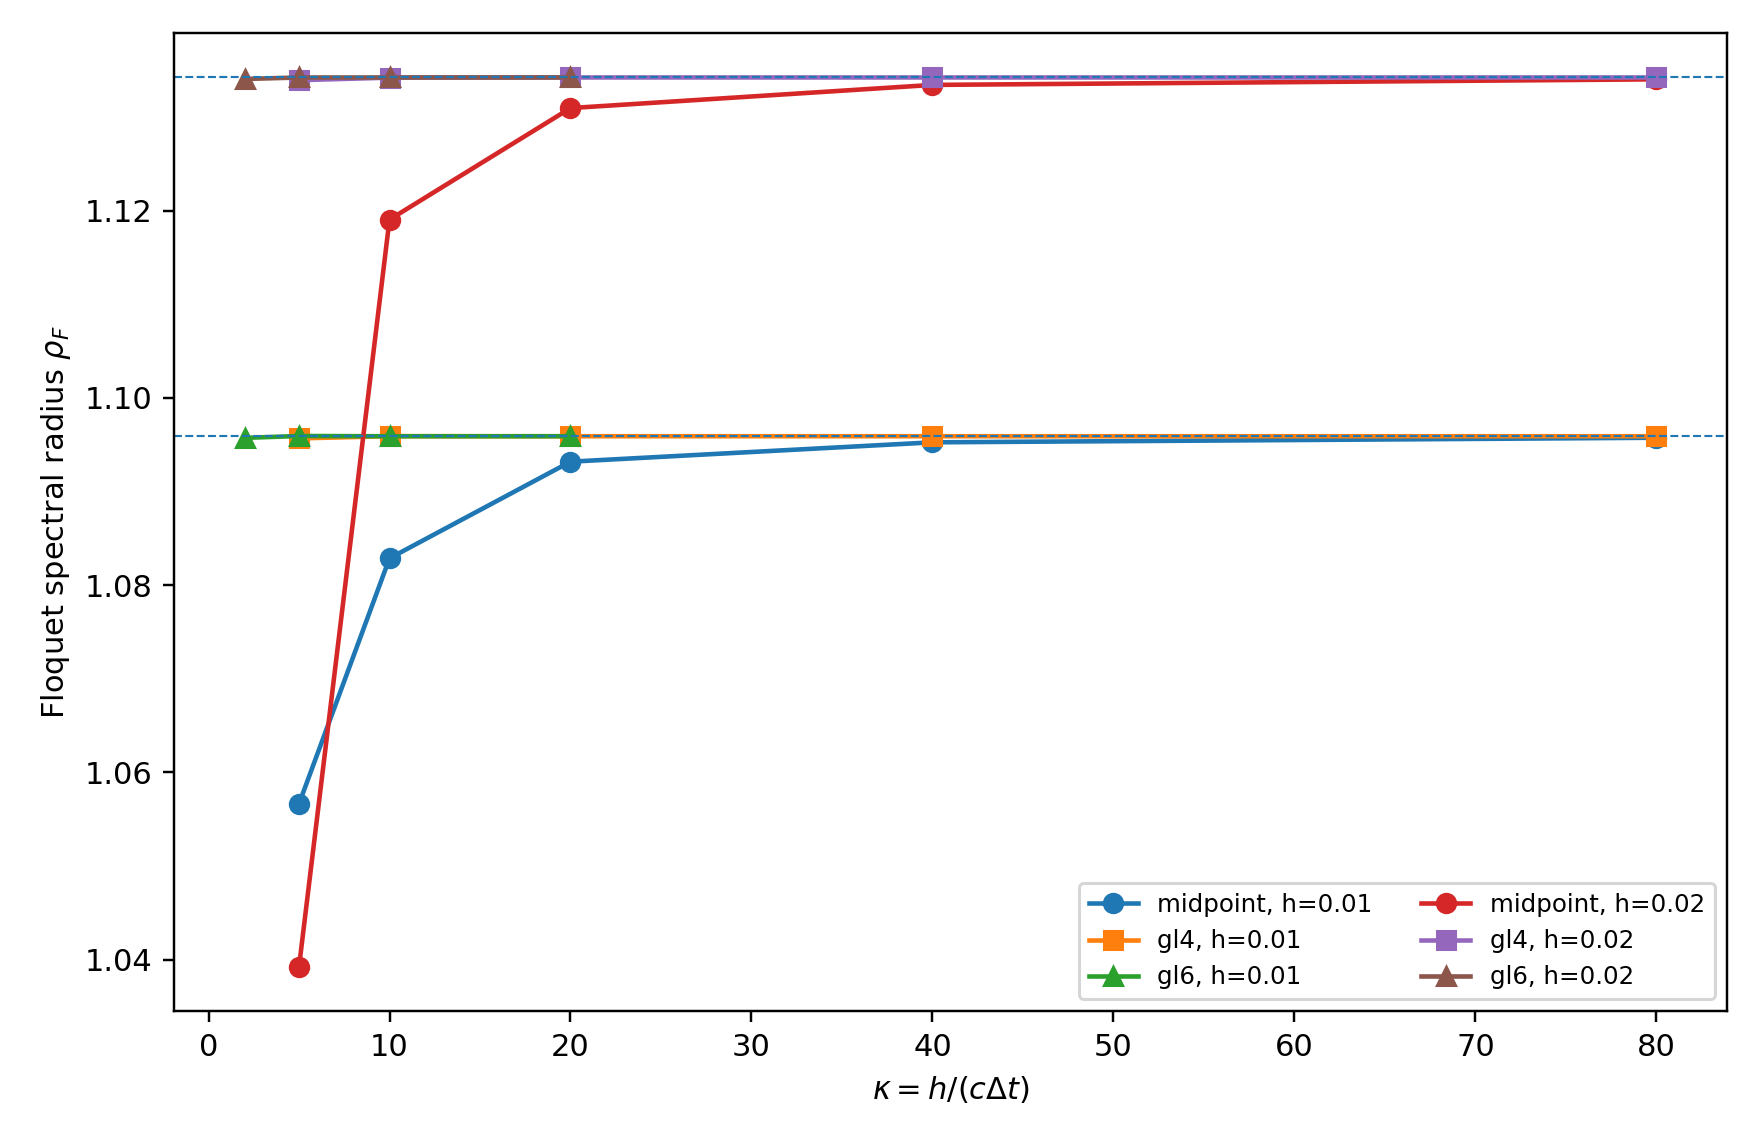
\includegraphics[width=0.76\textwidth]{wp3_floquet_three_integrators.png}
 \caption{Convergence of the one-cell Floquet spectral radius under midpoint,
 GL4, and GL6 time integration.  The high-order methods converge to the same
 unstable semidiscrete limit, while coarse midpoint integration can strongly
 attenuate the growth rate and change the dominant Floquet branch.}
 \label{fig:time-floquet}
\end{figure}

The midpoint spectral-radius error converges with observed order approximately
two, while GL4 converges with order approximately four until the nonlinear
fixed-point and Ritz tolerances set the numerical floor.  GL6 independently
confirms the limiting spectra.  Richardson extrapolations of GL4 and GL6 differ
by only $3.3\times10^{-7}$ for $h=0.01$ and $2.3\times10^{-7}$ for
$h=0.02$; independently extrapolated midpoint values agree within about
$2\times10^{-6}$.

\subsection{Method-dependent velocity correction}

For a free Nyquist solitary wave, the semidiscrete prediction is
$v_{\rm sd}=(A/h^2)V_h$.  Propagating the independently computed profile $F_h$
with the three integrators shows that the temporal similarity variable is
\begin{equation}
 \chi=\frac{A\Delta t}{h^3}=\frac{A/h^2}{\kappa}.
\end{equation}
For $A/h^2=0.1$, the observed convergence orders of the velocity are
$1.995$, $3.951$, and $5.931$ for midpoint, GL4, and GL6, respectively.  The
results for $h=0.01$ and $h=0.02$ collapse onto common curves.

Over the ranges used below, deterministic least-squares calibration gives
\begin{align}
 \frac{v_{\rm MP}}{v_{\rm sd}}-1
 &=-11.659289\chi^2+452.119772\chi^4
   -2.10497\times10^4\chi^6+O(\chi^8),
 \label{eq:mp-correction-new}\\
 \frac{v_{\rm GL4}}{v_{\rm sd}}-1
 &=-44.079876\chi^4+719.228502\chi^6
   +8148.209713\chi^8+O(\chi^{10}),
 \label{eq:gl4-correction}\\
 \frac{v_{\rm GL6}}{v_{\rm sd}}-1
 &=-116.356187\chi^6+1724.135317\chi^8+O(\chi^{10}).
 \label{eq:gl6-correction}
\end{align}
The calibration ranges are $\chi\le0.036$, $0.050$, and $0.050$,
respectively.  The leading powers agree with the formal orders of the methods;
the higher coefficients are used only as local numerical calibrations over
these ranges.

\begin{figure}[t]
 \centering
 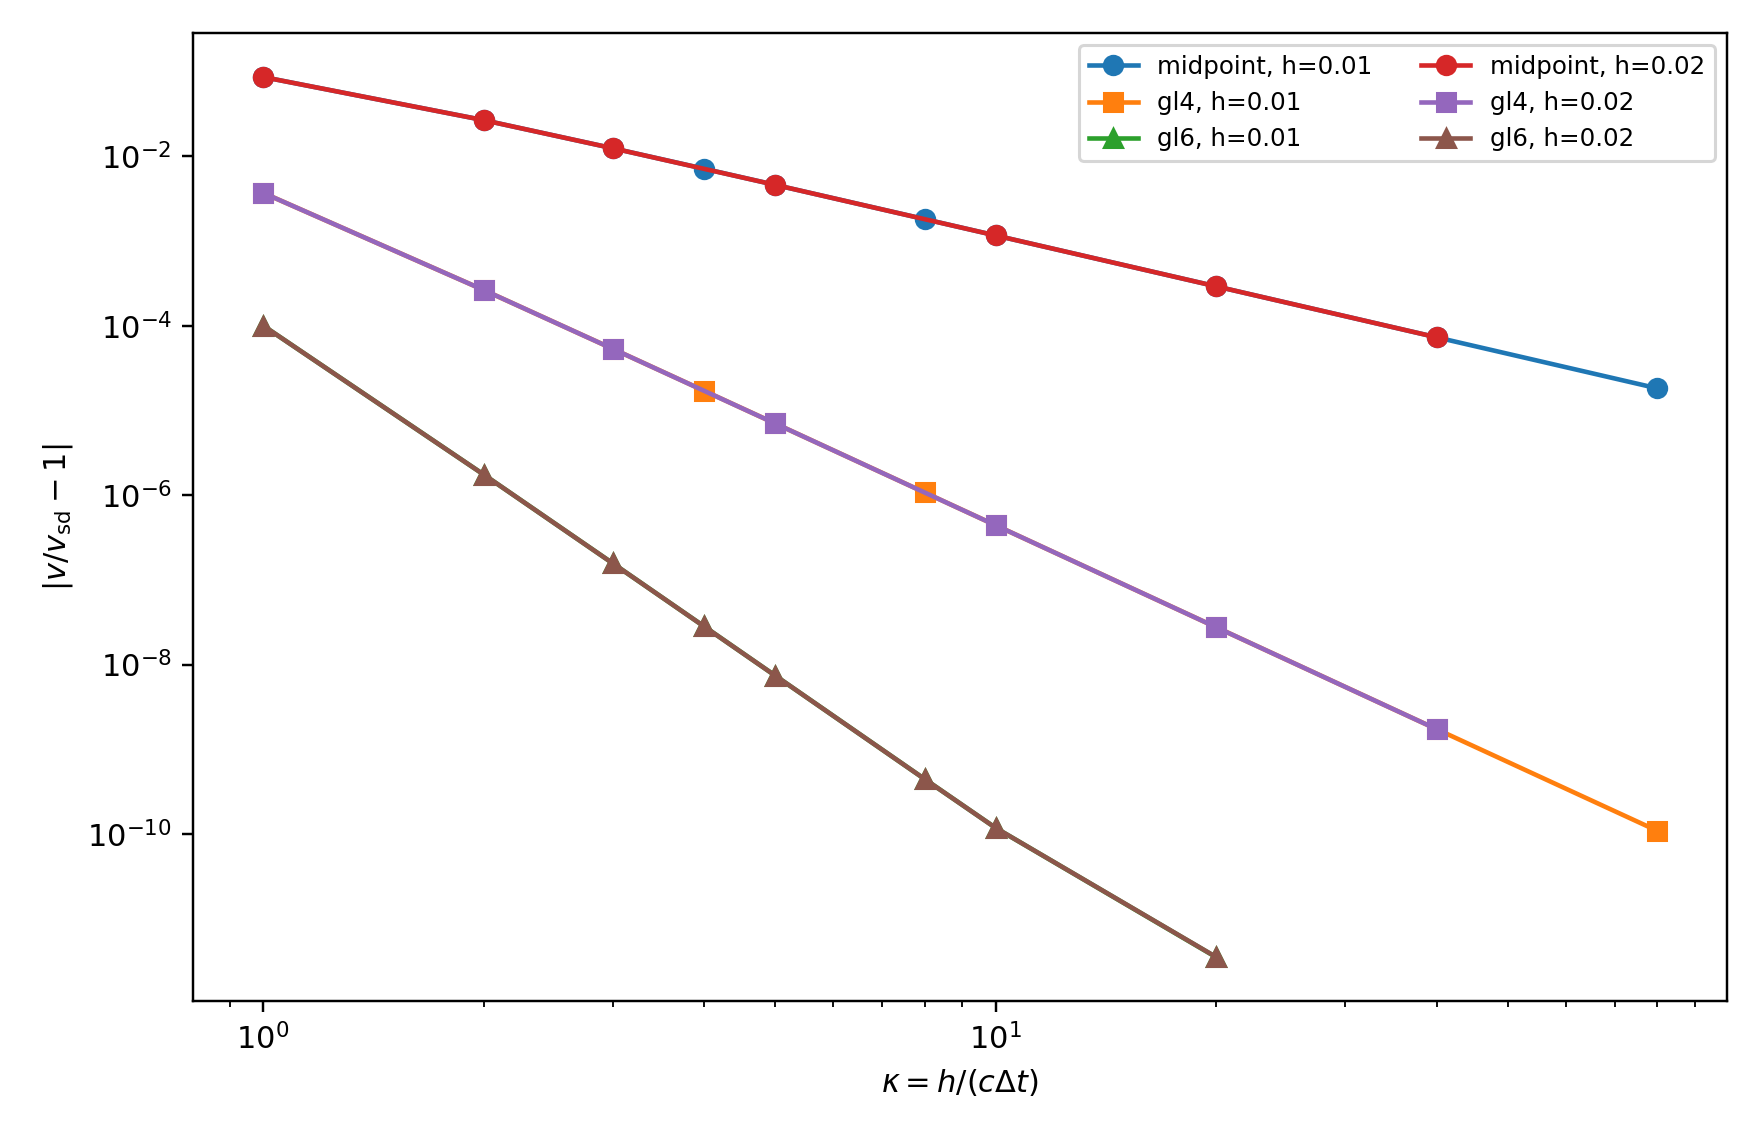
\includegraphics[width=0.76\textwidth]{wp3_velocity_order_three_integrators.png}
 \caption{Temporal convergence of the velocity of a free Nyquist solitary wave
 with $A/h^2=0.1$.  The observed orders are approximately two, four, and six.}
 \label{fig:time-velocity-order}
\end{figure}

\subsection{Independent nonlinear validation}

The velocity laws are tested on packets that were not used in the calibration.
For the two archived midpoint packets, Eq.~\eqref{eq:mp-correction-new} reduces
the deterministic relative discrepancies to $6.7\times10^{-6}$ and
$2.2\times10^{-6}$.  A natural GL4 evolution of the analytic compacton
spontaneously produces two clean packets.  They have
\begin{equation}
 \frac{A_1}{h^2}=0.1710967,\qquad v_1=3.5349106,
 \qquad
 \frac{A_2}{h^2}=0.0590858,\qquad v_2=1.2208014,
\end{equation}
with median fixed-profile residuals $1.2\times10^{-5}$ and
$2.4\times10^{-6}$.  Equation~\eqref{eq:gl4-correction} predicts their
velocities with deterministic relative discrepancies below $10^{-7}$.  Thus a
second time integrator both exhibits Nyquist shedding and produces packets
captured by the same semidiscrete solitary-wave family.

\begin{table}[t]
 \centering
 \caption{Out-of-sample validation of the fully discrete velocity laws.}
 \label{tab:time-packet-validation}
 \begin{tabular}{lcc}
 \toprule
 Packet & baseline relative error & calibrated relative error\\
 \midrule
 midpoint, $h=0.01$, $\kappa=5$  & $-1.16\times10^{-3}$ & $+6.65\times10^{-6}$\\
 midpoint, $h=0.02$, $\kappa=20$ & $-6.80\times10^{-5}$ & $+2.18\times10^{-6}$\\
 natural GL4 packet I             & $-5.92\times10^{-5}$ & $+7.82\times10^{-8}$\\
 natural GL4 packet II            & $-8.01\times10^{-7}$ & $+5.68\times10^{-8}$\\
 \bottomrule
 \end{tabular}
\end{table}

The detailed chronology and multiplicity of nonlinear shedding remain
integrator dependent.  The integrator-independent conclusions are the
existence of the unstable time-refined edge spectrum and the common
semidiscrete Nyquist solitary-wave family; the finite-$\Delta t$ multiplier and
packet velocity are method dependent.

\subsection{Accuracy-normalized cost}

In the reference implementation at $h=0.02$ and $N=800$, banded GL4 at
$\kappa=10$ requires approximately $0.038$ s per cell crossing and has
$|\rho_F-\rho_{F,\rm ref}|=1.7\times10^{-5}$.  Banded midpoint at
$\kappa=80$ requires approximately $0.062$ s and has error
$2.0\times10^{-4}$.  Generic sparse GL6 at $\kappa=5$ requires
approximately $0.059$ s and has error below $2\times10^{-6}$.  Although these timings are implementation dependent, they
show that the higher-stage methods can be more efficient at fixed spectral or
wave-speed accuracy because they require far fewer timesteps per cell crossing.
%%%%%%%%%%%%%%%%%%%%%%%%%%%%%%%%%%%%%%%%%%%%%%%%%%%%%%%%%%%%%%%%%%%%%%%%%%%%%%%
